\documentclass[a4paper]{article}

%% Language and font encodings
\usepackage[french]{babel}
\usepackage[utf8x]{inputenc}
\usepackage[T1]{fontenc}

%% Sets page size and margins
\usepackage[a4paper,top=3cm,bottom=3cm,left=2cm,right=2cm,marginparwidth=2cm]{geometry}
%% Useful packages
\usepackage{amsmath}
\usepackage{graphicx}
\usepackage[colorinlistoftodos]{todonotes}
\usepackage[colorlinks=true, allcolors=black]{hyperref}
\usepackage{fourier-orns}
\usepackage{titlesec}
\usepackage{fancyhdr}
\usepackage{fancyvrb}
%\renewcommand{\thefootnote}{\*}
\pagestyle{fancy} 
\setcounter{tocdepth}{5}

%% Tikz stuff
\usepackage{tikz}
\usetikzlibrary{calc, arrows}
\tikzstyle{incolore} = [rectangle, rounded corners, draw=black, minimum height=1cm, minimum width=3cm, text width=3cm, text centered]

\usepackage{libertine}
\newcommand{\hsp}{\hspace{20pt}}
\newcommand{\HRule}{\rule{\linewidth}{0.5mm}}

\renewcommand{\headrulewidth}{1pt}
\fancyhead[C]{}
\fancyhead[L]{}
\fancyhead[R]{\footnotesize{\scshape Introduction aux bases de données}}

\renewcommand{\footrulewidth}{1pt}
\fancyfoot[C]{}
\fancyhead[L]{}
\fancyfoot[R]{\thepage}

\definecolor{Zgris}{rgb}{0.87,0.85,0.85}

\usepackage{eso-pic,graphicx}
\usepackage{xcolor}
\newcommand{\bgimg}[1]{
\AddToShipoutPicture
    {
        \put(\LenToUnit{0 cm},\LenToUnit{0 cm})
        {
            \includegraphics[width=\paperwidth,height=\paperheight]{#1}
        }
    }
}
\begin{document}




%%\bgimg{Image_15.jpg}

















\begin{titlepage}
    \begin{sffamily}
        \begin{center}

            
\includegraphics[width=5cm]{images/LogoHenallux.PNG}~\\[1.5cm]
            \textsc{\Large Travail d'évaluation}\\[1.5cm]

            \HRule \\[0.4cm]
            { \huge \bfseries Schéma relationnel\\[0.4cm] }
            \HRule \\[2cm]

            \begin{minipage}{0.4\textwidth}
                \begin{flushleft} \large
                    Roumache Grégoire\\
                    Sécurité des systèmes\\
                    Première année, groupe H \\
                \end{flushleft}
            \end{minipage}
            \begin{minipage}{0.55\textwidth}
            \begin{flushright} \large
                Introduction aux bases de données\\
                Hénallux\\
                Année académique 2019-2020\\
            \end{flushright}
            \end{minipage}
            \vfill

            {\large 27 Avril 2020}
        \end{center}
    \end{sffamily}
\end{titlepage}







\let\cleardoublepage\clearpage















\begin{center}
    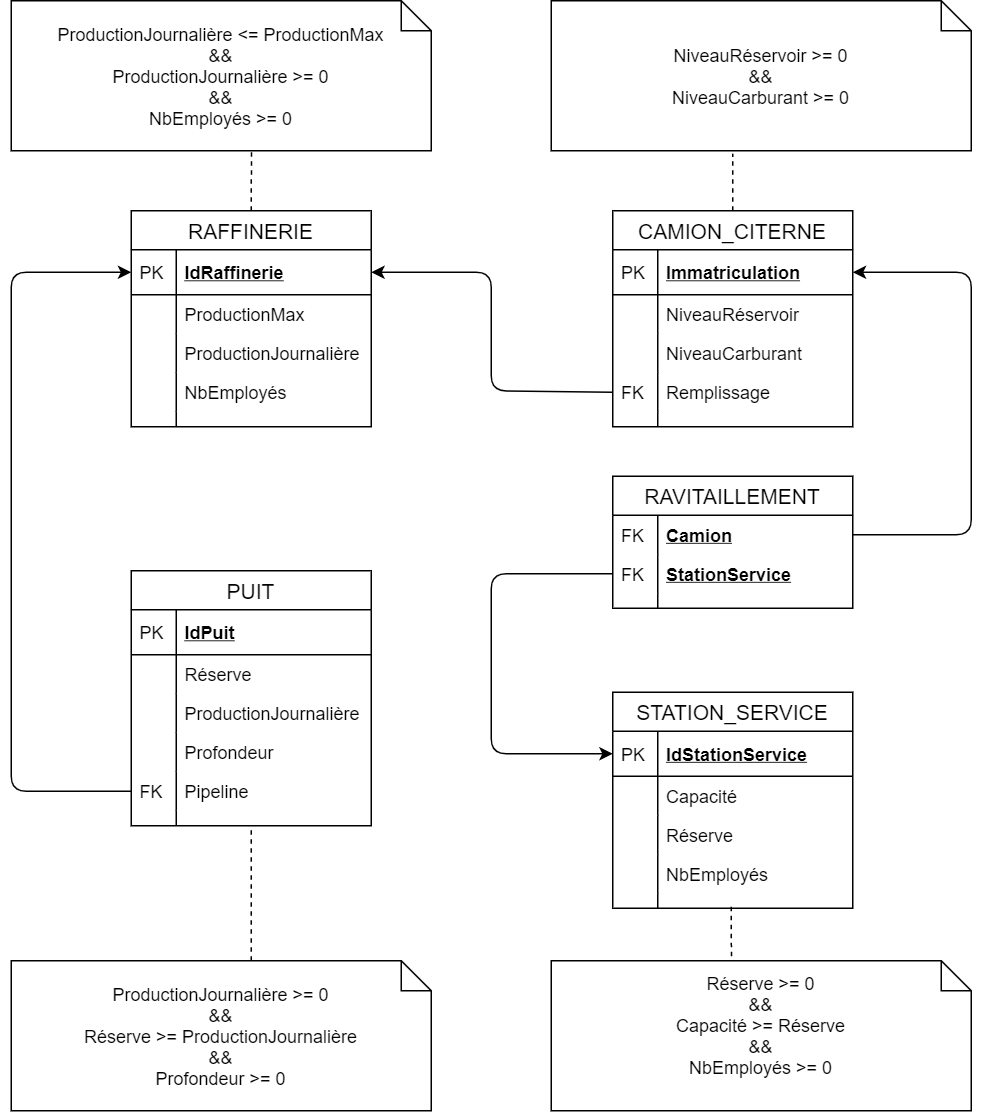
\includegraphics[width=0.99\textwidth]{images/RoumacheGregoire_rel.png}
\end{center}

\textbf{Remarque:} l'entité RAVITAILLEMENT sert à faire la liaison entre les entités CAMION\_CITERNE et \\ STATION\_SERVICE. Ses attributs sont marqués comme des clés étrangères (FK) mais lui servent aussi de clé primaire composée, c'est pour ça qu'ils sont soulignés.



















\end{document}
